\chapter{Testing}


\section{NAND}

\section{NOR2}

\section{XOR2}

\section{DFF}

TEST CIRCUIT

FUNCTIONALITY TESTING 

SPEED TESTING

LAYOUT VS SCHEMATIC 

ERRONIOUS BEHAVIOUR


\begin{figure}[h]  
\centering
   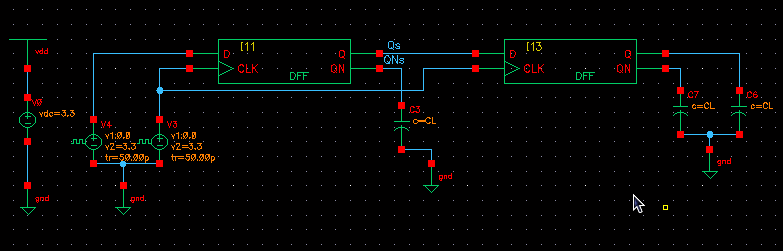
\includegraphics[width=0.45\textwidth]{Figures/DFFTestSchem.png}
\caption{DFF Test Circuit Schematic.}
\label {fig:DFFTestSchem}
\end{figure}

\section{Duel Edge Triggered Flip Flop}

\begin{figure}[h]  
\centering
   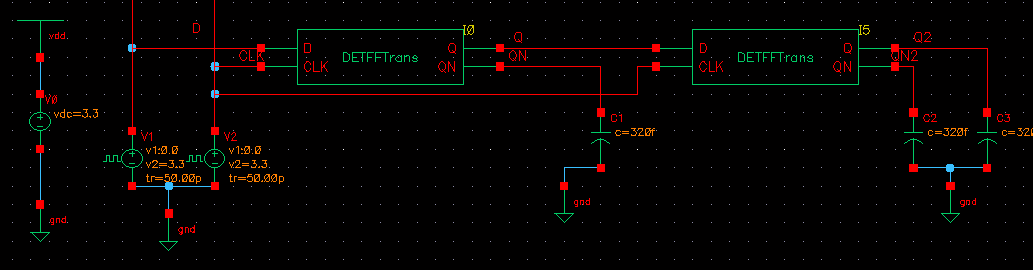
\includegraphics[width=0.45\textwidth]{Figures/DETFFTestSchem.png}
\caption{DETFF Test Circuit Schematic.}
\label {fig:DETFFTestSchem}
\end{figure}

\section{C Element}

\section{Dual Rail AND}

TEST CIRCUIT

\begin{figure}[h]  
\centering
   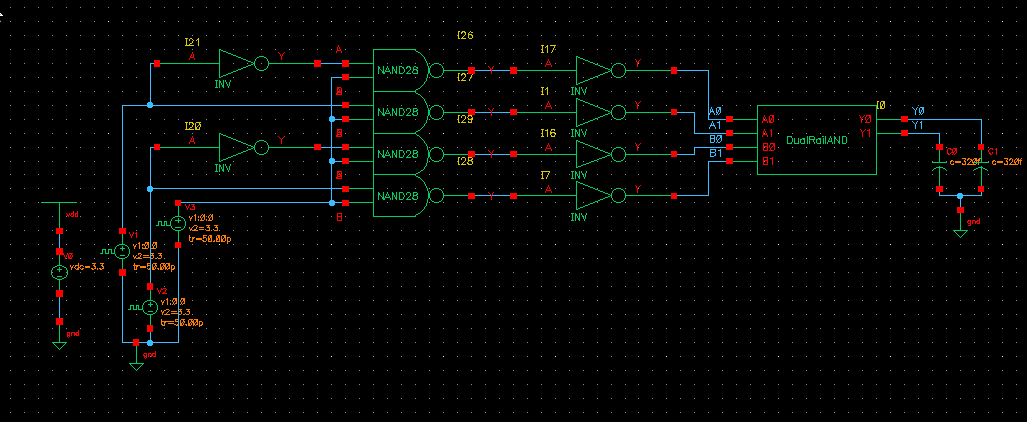
\includegraphics[width=0.45\textwidth]{Figures/DualRailANDTestSchem.png}
\caption{Dual Rail AND Test Schematic.}
\label {fig:DualRailANDTestSchem}
\end{figure}

FUNCTIONALITY TESTING 

\begin{figure}[h]  
\centering
   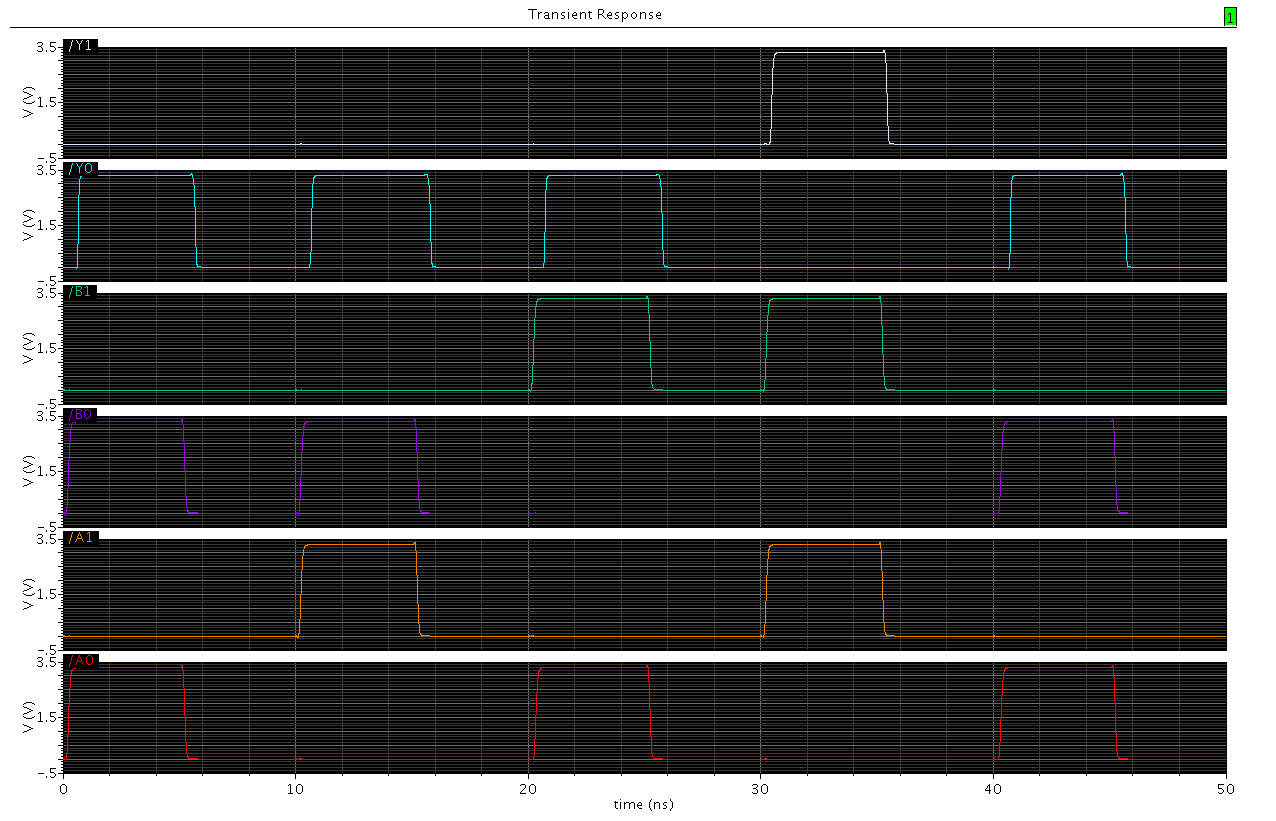
\includegraphics[width=0.45\textwidth]{Figures/DualAndCorrectOperation.png}
\caption{Dual Rail AND Simulation showing correct operation.}
\label {fig:DualAndCorrectOperation}
\end{figure}

SPEED TESTING

LAYOUT VS SCHEMATIC 

ERRONIOUS BEHAVIOUR







\section{1-bit Subtractor}

\section{2-to-1 Multiplexor}

\section{Mutex Element}
